\documentclass{beamer}
\usepackage{amssymb,amsmath,amsthm}
\usepackage{color}
\usepackage{subfig}
\usepackage[]{graphicx}
\usepackage[]{bm}
\usepackage{xcolor}
\usepackage[mathscr]{eucal}
\usepackage{epsfig}


\mode<presentation>
{
\usetheme{Ilmenau}
\usecolortheme{beaver}
}

\title{Applications of Structured Learning to Polyphonic Transcription}
\author[]{J. Shi and C. Herrmann}
\institute[]{Presented for Advanced Topics in Machine Learning}

\makeindex

\begin{document}
\begin{frame}{}
\titlepage
Using structured learning to transcribe piano music
\end{frame}

\AtBeginSection[]
{
\begin{frame}
\frametitle{Outline}
\tableofcontents[currentsection]
\end{frame}
}


\section{Motivation}
\begin{frame}{Example}
Please listen to the following selections.
\end{frame}

\begin{frame}{The Problem}

{\bf Goal:} Given a recording of a song, transcribe the song in an accurate manner.\\
\vspace{.5cm}
{\bf Input:} Recording of song taken in variable settings and with variable quality of recording equipment.\\
\vspace{.1cm}
{\bf Output:} MIDI file of the song.
\end{frame}

\section{Previous Solutions}
\begin{frame}{Previous Solutions}

The general appraoch

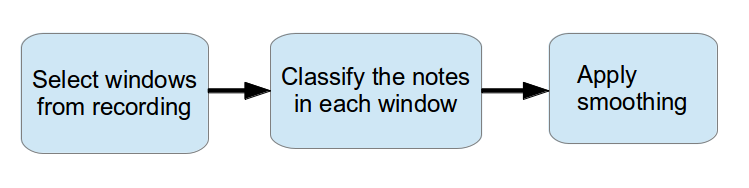
\includegraphics[scale=.4]{algorithm_template.png}

Some separate the classification of notes into two steps: note onset detection and then classification of notes. These tend to suffer, why?
\end{frame}

\begin{frame}{Previous Solutions}
Lots of variations and possibilities to consider
\begin{itemize}
\item How to select the windows? Overlapping? Multiple windows with different lengths?
\item What classification technique to use? How to extract feature vector from windows?
\item What smoothing technique should be applied? How much should this encompass.
\end{itemize}
\end{frame}

\begin{frame}{Previos Solutions}
Three general styles of classification
\begin{itemize}
\item Discriminative - uses SVM one versus all classifiers
\item Generative/Recursive Neural Nets - TODO
\item F0 approach - TODO
\end{itemize}
\end{frame}

\section{Algorithm}
\begin{frame}{Idea}
So far the descriminative approaches have performed the best.
\pause
A couple of thoughts:
\begin{itemize}
\item One-versus-All SVM is terrible!
\item Why place too much emphasis upon the HMM at end?
\item Can improve the feature vectors chosen and the way windowing is done.
\end{itemize}
\end{frame}


\begin{frame}{New System}
\end{frame}
\begin{frame}{Benefits}
\end{frame}

\section{Preliminary Results}
\begin{frame}
\end{frame}

\section{Summary}
\begin{frame}
\end{frame}

\section{References}
\begin{frame}{Bibliography}
\bibliographystyle{amsalpha}
\nocite{*}
\bibliography{pres}
\end{frame}
\end{document}
